% Provenance (never printed): cycle 2 "Questionner l'espace et le temps ---
% se situer dans l'espace": representations of familiar spaces (plans), "lire
% des plans, se reperer sur des cartes. Elements constitutifs d'une carte :
% titre, echelle, orientation, legende"; see sources/book1/PROVENANCE.md.
% Book 1, grade 2, chapter 2. Sync 1: "scale" is owned here; "cardinal
% directions" is the physics series' term (prose only); "compass rose" here.
\chapter{Dari Gambar ke Peta}\label{ch:g2:drawing-to-map}

Seekor burung merpati terbang di atas sekolah. Apa yang dilihatnya? Bukan
pintu depan, bukan jendela, bukan wajah anak-anak: dari atas sana ia hanya
melihat bagian atas benda-benda. Atap-atap gedung berupa persegi panjang
kelabu. Halaman sekolah berupa bentuk besar yang kosong dengan beberapa
puncak pohon yang bundar. Jalan-jalan setapak berupa garis tipis. Merpati
itu melihat sekolah dari atas --- seperti yang ditunjukkan sebuah \omterm{def:g2:drawing-to-map:map}{peta}.

\begin{omfigure}
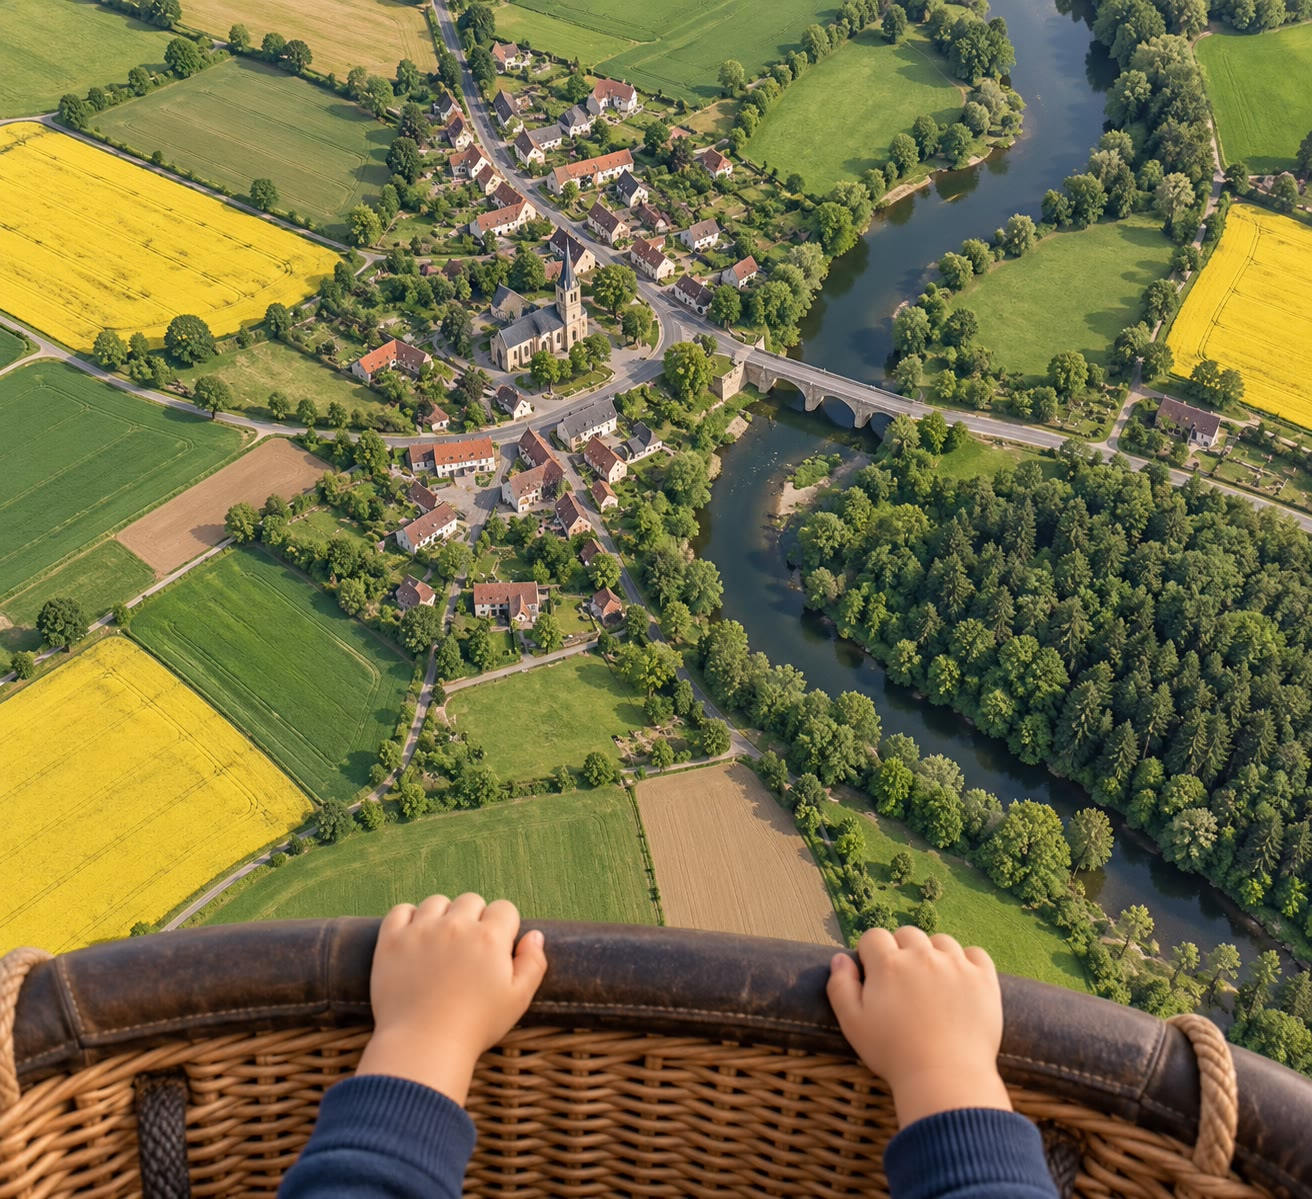
\includegraphics[width=0.62\linewidth]{images/book1/ai/g2-balloon-view.jpg}

{\small Pedesaan yang dilihat dari balon udara: ladang, desa, jalan, \omterm{def:g1:landscapes-around-us:water}{sungai}
dan jembatannya, semuanya dilihat dari atas.}
\end{omfigure}

\section{Dilihat dari samping, dilihat dari atas}

Letakkan beberapa balok mainan di atas meja. Lihatlah balok-balok itu dari
samping: kamu melihat tingginya, dan balok yang di belakang tersembunyi di
balik balok yang di depan. Sekarang berdirilah dan lihatlah balok-balok itu
dari atas: kamu tidak lagi melihat seberapa tinggi balok-balok itu, tetapi
kamu melihat dengan tepat letak setiap balok, dan seberapa jauh jaraknya
satu sama lain.

\begin{omfigure}
\begin{tikzpicture}[x=1cm, y=1cm, font=\small]
  % side view
  \begin{scope}
    \draw[black!50] (-0.2,0) -- (4.6,0);
    \fill[red!55, draw=black!60] (0.2,0) rectangle (1.2,1.6);
    \fill[ocBlue!55, draw=black!60] (1.6,0) rectangle (3.0,0.8);
    \fill[yellow!70, draw=black!60] (3.4,0) -- (3.9,1.1) -- (4.4,0) -- cycle;
    \node at (2.2,-0.5) {dilihat dari samping};
  \end{scope}
  % from above
  \begin{scope}[shift={(6.4,0)}]
    \draw[black!30, fill=black!3] (-0.2,-0.1) rectangle (4.6,2.3);
    \fill[red!55, draw=black!60] (0.2,0.4) rectangle (1.2,1.4);
    \fill[ocBlue!55, draw=black!60] (1.6,1.0) rectangle (3.0,2.0);
    \fill[yellow!70, draw=black!60] (3.9,0.75) circle (0.5);
    \node at (2.2,-0.5) {dilihat dari atas};
  \end{scope}
\end{tikzpicture}

{\small Tiga balok di atas meja: balok merah yang tinggi, balok biru yang
pipih, dan kerucut kuning. Dari atas, kerucut itu tampak sebagai lingkaran
dan balok yang tinggi tampak sebagai persegi.}
\label{fig:g2:drawing-to-map:blocks}
\end{omfigure}

\begin{definition}[Denah]\label{def:g2:drawing-to-map:plan}
Yang disebut \emph{denah}\index{denah} adalah gambar sebuah tempat yang
kecil --- sebuah ruangan, rumah, sekolah, kebun --- seperti yang terlihat
tegak lurus dari atas, digambar lebih kecil daripada aslinya tetapi dengan
setiap bagian di tempatnya yang benar.
\end{definition}

\section{Menggambar lebih kecil: skala}

Ruang kelas terlalu besar untuk digambar di selembar kertas dengan ukuran
aslinya. Kita menggambarnya lebih kecil --- tetapi setiap bagian harus
diperkecil dengan cara yang sama, kalau tidak \omterm{def:g2:drawing-to-map:plan}{denahnya} akan berbohong. Cara
yang paling mudah adalah memakai kertas berpetak: satu kotak di kertas
mewakili satu meter di ruang kelas.

\begin{definition}[Skala]\label{def:g2:drawing-to-map:scale}
Yang disebut \emph{skala}\index{skala} sebuah \omterm{def:g2:drawing-to-map:plan}{denah} atau \omterm{def:g2:drawing-to-map:map}{peta} menyatakan
berapa kali gambar itu lebih kecil daripada tempat yang sebenarnya: berapa
jauh jarak di permukaan tanah yang diwakili oleh suatu panjang pada gambar.
Misalnya: \emph{1 kotak mewakili 1 meter}.
\end{definition}

\begin{omfigure}
\begin{tikzpicture}[x=0.75cm, y=0.75cm, font=\scriptsize]
  \draw[black!15] (0,0) grid (10,8);
  \draw[black, line width=1.6pt] (0,0) rectangle (10,8);
  % board on the north wall
  \fill[black!70] (3,7.8) rectangle (7,8);
  % teacher's desk
  \fill[brown!50, draw=black!70] (4,6) rectangle (6,7);
  % pupils' desks: 3 rows of 3
  \foreach \x in {1,4,7} \foreach \y in {1,2.5,4}
    \fill[orange!45, draw=black!70] (\x,\y) rectangle ++(2,1);
  % cupboard
  \fill[ocBlue!40, draw=black!70] (9,5) rectangle (10,8);
  % door (gap) on the east wall, windows on the west wall
  \fill[white] (9.85,1) rectangle (10.15,2);
  \draw[black!70] (10,2) arc[start angle=90, end angle=180, radius=1];
  \foreach \y in {1.5,4.5}
    \draw[ocBlue, line width=2.5pt] (0,\y) -- (0,\y+2);
  % legend
  \begin{scope}[shift={(11,7.2)}]
    \node[anchor=west, font=\small\bfseries] at (0,0.4) {Ruang kelas};
    \fill[black!70] (0,-0.25) rectangle (0.8,-0.05); \node[anchor=west] at (1,-0.15) {papan tulis};
    \fill[brown!50, draw=black!70] (0,-1.1) rectangle (0.8,-0.7); \node[anchor=west] at (1,-0.9) {meja guru};
    \fill[orange!45, draw=black!70] (0,-1.85) rectangle (0.8,-1.45); \node[anchor=west] at (1,-1.65) {meja murid};
    \fill[ocBlue!40, draw=black!70] (0,-2.6) rectangle (0.8,-2.2); \node[anchor=west] at (1,-2.4) {lemari};
    \draw[ocBlue, line width=2.5pt] (0,-3.15) -- (0.8,-3.15); \node[anchor=west] at (1,-3.15) {jendela};
    \draw[black!70] (0.8,-3.95) arc[start angle=0, end angle=90, radius=0.6]; \draw[black, line width=1.6pt] (0.2,-3.95) -- (0.8,-3.95); \node[anchor=west] at (1,-3.7) {pintu};
    \draw[black!15] (0,-4.9) rectangle (0.75,-4.15);
    \node[anchor=west] at (1,-4.53) {1 kotak = 1 meter};
    \pic[scale=0.7, transform shape] at (0.7,-6.2) {compassrose};
  \end{scope}
\end{tikzpicture}

{\small \omterm{def:g2:drawing-to-map:plan}{Denah} sebuah ruang kelas di kertas berpetak, dengan judul, \omterm{def:g2:drawing-to-map:legend}{legenda},
\omterm{def:g2:drawing-to-map:scale}{skala}, dan \omterm{def:g2:drawing-to-map:directions}{mawar anginnya}. Dinding utara, tempat papan tulis, ada di bagian
atas.}
\label{fig:g2:drawing-to-map:classroom}
\end{omfigure}
% (exercise data: an invented classroom of 10 m by 8 m)

\begin{method}[Mengukur pada denah]\label{met:g2:drawing-to-map:measure}
Untuk mencari panjang sebenarnya pada \omterm{def:g2:drawing-to-map:plan}{denah} yang digambar di atas kotak-kotak:
\begin{enumerate}
  \item hitunglah kotak-kotak sepanjang garis yang kamu inginkan;
  \item bacalah \omterm{def:g2:drawing-to-map:scale}{skalanya}: berapa yang diwakili oleh satu kotak;
  \item berikan jawabannya dalam meter (atau dalam kilometer pada \omterm{def:g2:drawing-to-map:map}{peta}).
\end{enumerate}
\end{method}

\begin{example}[Berapa panjang ruang kelas itu?]\label{ex:g2:drawing-to-map:length}
Sepanjang dinding utara pada \omterm{def:g2:drawing-to-map:plan}{denah} ada 10 kotak. Satu kotak mewakili 1
meter, jadi panjang ruang kelas itu 10 meter. Sepanjang dinding barat ada 8
kotak: lebarnya 8 meter. Papan tulis menempati 4 kotak dinding utara:
panjangnya 4 meter.
\end{example}

\begin{omfigure}
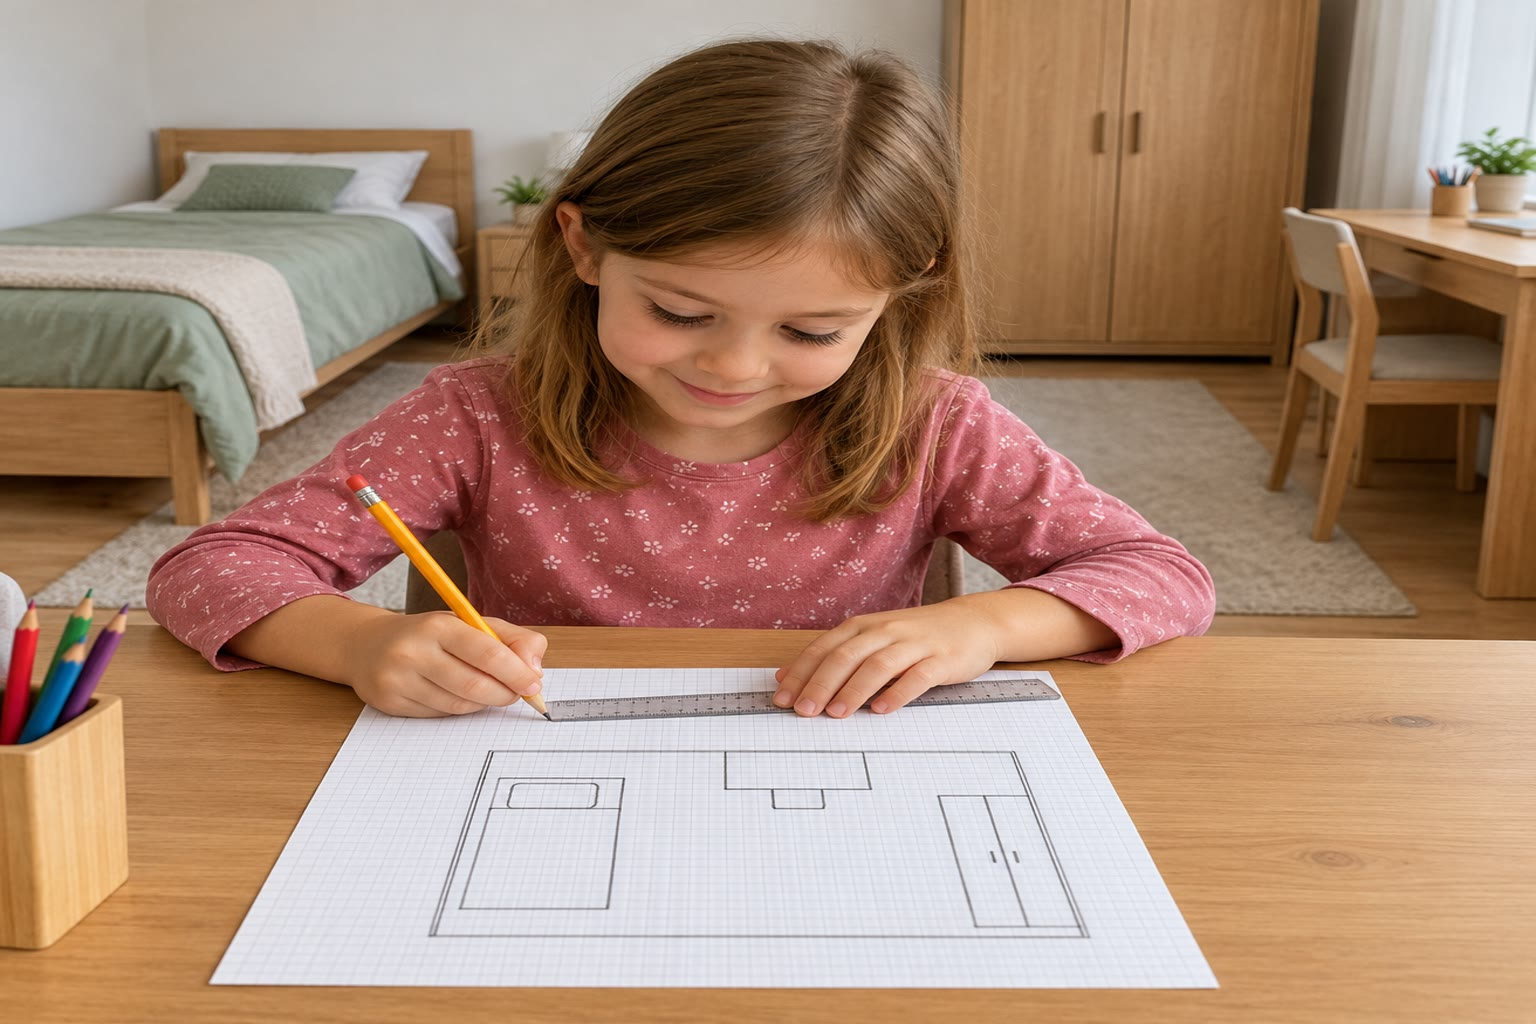
\includegraphics[width=0.55\linewidth]{images/book1/ai/g2-bedroom-plan.jpg}

{\small Menggambar \omterm{def:g2:drawing-to-map:plan}{denah} sebuah kamar tidur di kertas berpetak.}
\end{omfigure}

\section{Dari denah ke peta}

\omterm{def:g2:drawing-to-map:plan}{Denah} menunjukkan sebuah tempat yang kecil. Ketika kita menggambar tempat
yang lebih besar --- seluruh kota, sebuah \omterm{def:g1:landscapes-around-us:landform}{lembah}, sebuah negara --- kita
menggambar \omterm{def:g2:drawing-to-map:map}{peta}.

\begin{definition}[Peta]\label{def:g2:drawing-to-map:map}
Yang disebut \emph{peta}\index{peta} adalah gambar sebagian besar
permukaan Bumi, yang dilihat dari atas dan digambar jauh lebih kecil
daripada aslinya.
\end{definition}

Pada \omterm{def:g2:drawing-to-map:map}{peta}, sebuah rumah terlalu kecil untuk digambar seperti aslinya, jadi
para pembuat \omterm{def:g2:drawing-to-map:map}{peta} memakai tanda-tanda kecil: sebuah titik untuk pertanian,
garis biru untuk \omterm{def:g1:landscapes-around-us:water}{sungai}, bentuk hijau untuk hutan kecil. Arti setiap tanda
diberikan dalam kotak di samping \omterm{def:g2:drawing-to-map:map}{peta}.

\begin{definition}[Legenda]\label{def:g2:drawing-to-map:legend}
Yang disebut \emph{simbol peta}\index{simbol peta} adalah tanda kecil yang
mewakili satu jenis benda pada \omterm{def:g2:drawing-to-map:plan}{denah} atau \omterm{def:g2:drawing-to-map:map}{peta}. Yang disebut
\emph{legenda}\index{legenda} adalah kotak yang menunjukkan setiap simbol
pada \omterm{def:g2:drawing-to-map:map}{peta} beserta artinya.
\end{definition}

\section{Menemukan jalan: empat arah dan mawar angin}

Untuk menyatakan letak sesuatu, ``di kiri'' atau ``di kanan'' tidak cukup:
apa yang ada di sebelah kirimu berada di sebelah kanan orang yang
menghadapmu. Orang memakai empat arah yang sama bagi semua orang: utara,
timur, selatan, dan barat. Kamu sudah mengenalnya di buku fisika, bersama
kompas. Pada pagi hari Matahari terbit di timur, dan pada sore hari
Matahari terbenam di barat; utara dan selatan berada di tengah-tengah di
antara keduanya, saling berhadapan.

\begin{omfigure}
\begin{tikzpicture}[font=\small]
  \pic[scale=1.5, transform shape] at (0,0) {compassrose};
  \node[align=left, anchor=west, font=\small] at (2.6,0.3)
    {U = utara (di bagian atas kebanyakan peta)\\T = timur (di kanan)\\S = selatan (di bawah)\\B = barat (di kiri)};
\end{tikzpicture}

{\small Sebuah \omterm{def:g2:drawing-to-map:directions}{mawar angin}. Di antara utara dan timur ada timur laut; di
antara selatan dan barat, barat daya.}
\label{fig:g2:drawing-to-map:rose}
\end{omfigure}

\begin{definition}[Mawar angin]\label{def:g2:drawing-to-map:directions}
Yang disebut \emph{mawar angin}\index{mawar angin} adalah gambar bintang
pada \omterm{def:g2:drawing-to-map:map}{peta} yang menunjukkan arah utara, timur, selatan, dan barat. Pada
kebanyakan \omterm{def:g2:drawing-to-map:map}{peta}, utara ada di atas, timur di kanan, selatan di bawah, dan
barat di kiri.
\end{definition}

\begin{safety}
Jangan pernah melihat Matahari untuk mencari arah timur atau barat: matamu
bisa rusak selamanya. Lihatlah bayang-bayang saja, atau pakailah kompas.
\end{safety}

\section{Membaca peta sungguhan}

Setiap \omterm{def:g2:drawing-to-map:map}{peta} yang baik mempunyai empat bagian: \textbf{judul} yang
menyatakan apa yang ditunjukkan \omterm{def:g2:drawing-to-map:map}{peta}, \textbf{\omterm{def:g2:drawing-to-map:legend}{legenda}}, \textbf{\omterm{def:g2:drawing-to-map:scale}{skala}}, dan
\textbf{\omterm{def:g2:drawing-to-map:directions}{mawar angin}} (atau setidaknya sebuah panah yang menunjuk ke utara).
Inilah \omterm{def:g2:drawing-to-map:map}{peta} sebuah \omterm{def:g1:landscapes-around-us:landform}{lembah} berbukit, Perbukitan Varden. \omterm{def:g1:landscapes-around-us:landform}{Lembah} rekaan ini
akan kamu jumpai berkali-kali dalam buku ini dan buku-buku berikutnya,
setiap kali digambar dengan lebih rinci.

\begin{omfigure}
\begin{tikzpicture}
\begin{axis}[width=9.6cm, scale only axis,
    xmin=0, xmax=10, ymin=0, ymax=8, axis equal image,
    xtick={0,...,10}, ytick={0,...,8}, xticklabels={}, yticklabels={},
    grid=major, grid style={black!20}, major tick length=0pt,
    axis background/.style={fill=green!12!omLithAlluv},
    title={\textbf{Perbukitan Varden}}]
  \addplot[fill=omHypsLandD, draw=omHypsLandE!80!black, line width=0.4pt, fill opacity=0.85,
    unbounded coords=jump, even odd rule] table {figdata/out/grade-2-varden_plan-hills.dat};
  \addplot[fill=green!45!black!55, draw=green!35!black, line width=0.4pt] table {figdata/out/grade-2-varden_plan-wood.dat};
  \addplot[ocBlue!85!black, line width=2.2pt] table {figdata/out/shared-region-river.dat};
  \addplot[red!65!black, line width=1.3pt] table {figdata/out/grade-2-varden_plan-road.dat};
  \fill[black] (axis cs:5.012,3.414) ++(-3pt,-4pt) rectangle ++(6pt,8pt);
  \fill[white] (axis cs:5.012,3.414) ++(-1.6pt,-4pt) rectangle ++(3.2pt,8pt);
  \fill[brown!70!black] (axis cs:2.5,3.5) ++(-3.5pt,-3.5pt) rectangle ++(7pt,7pt);
  \fill[red!70!black] (axis cs:7.5,5.5) ++(-5pt,-3pt) rectangle ++(4pt,4pt);
  \fill[red!70!black] (axis cs:7.5,5.5) ++(1pt,-3pt) rectangle ++(4pt,4pt);
  \fill[red!70!black] (axis cs:7.5,5.5) ++(-2pt,2pt) rectangle ++(4pt,4pt);
\end{axis}
\begin{scope}[shift={(10.2,6.4)}, font=\small]
  \node[anchor=west, font=\small\bfseries] at (-0.1,0.55) {Legenda};
  \fill[omHypsLandD, draw=omHypsLandE!80!black] (0,-0.2) rectangle (0.7,0.15); \node[anchor=west] at (0.85,0) {bukit};
  \fill[green!45!black!55] (0,-0.85) rectangle (0.7,-0.5); \node[anchor=west] at (0.85,-0.67) {hutan};
  \draw[ocBlue!85!black, line width=2.2pt] (0,-1.35) -- (0.7,-1.35); \node[anchor=west] at (0.85,-1.35) {sungai};
  \draw[red!65!black, line width=1.3pt] (0,-2.0) -- (0.7,-2.0); \node[anchor=west] at (0.85,-2.0) {jalan};
  \fill[black] (0.25,-2.8) rectangle (0.45,-2.5); \fill[white] (0.3,-2.8) rectangle (0.4,-2.5); \node[anchor=west] at (0.85,-2.65) {jembatan};
  \fill[brown!70!black] (0.23,-3.45) rectangle (0.47,-3.21); \node[anchor=west] at (0.85,-3.33) {pertanian};
  \foreach \dx/\dy in {0.12/-4.1, 0.33/-4.1, 0.22/-3.92}
    \fill[red!70!black] (\dx,\dy) rectangle ++(0.13,0.13);
  \node[anchor=west] at (0.85,-3.98) {desa};
  \draw[black!40] (0,-4.95) rectangle (0.5,-4.45); \node[anchor=west, align=left] at (0.85,-4.7) {1 kotak\\= 1 kilometer};
  \pic[scale=0.75, transform shape] at (0.8,-6.5) {compassrose};
\end{scope}
\end{tikzpicture}

{\small \omterm{def:g2:drawing-to-map:map}{Peta} sederhana Perbukitan Varden, dengan judul, \omterm{def:g2:drawing-to-map:legend}{legenda}, \omterm{def:g2:drawing-to-map:scale}{skala}, dan
\omterm{def:g2:drawing-to-map:directions}{mawar anginnya}. \omterm{def:g1:landscapes-around-us:water}{Sungainya} mengalir dari barat ke timur.}
\label{fig:g2:drawing-to-map:varden}
\end{omfigure}
% (figdata/grade-2/varden_plan.py; the region: figdata/shared/region.py)

\begin{method}[Membaca peta]\label{met:g2:drawing-to-map:read}
\begin{enumerate}
  \item Bacalah judulnya: tempat apa yang ditunjukkan \omterm{def:g2:drawing-to-map:map}{peta} itu?
  \item Bacalah \omterm{def:g2:drawing-to-map:legend}{legendanya}: apa arti setiap simbol?
  \item Carilah \omterm{def:g2:drawing-to-map:directions}{mawar anginnya}: di mana arah utara?
  \item Bacalah \omterm{def:g2:drawing-to-map:scale}{skalanya}, dan hitunglah kotak-kotak untuk mencari jarak.
\end{enumerate}
\end{method}

\begin{example}[Dari pertanian ke desa]\label{ex:g2:drawing-to-map:farm}
Pada \omterm{def:g2:drawing-to-map:map}{peta} Perbukitan Varden, pertanian itu terletak di sebelah selatan
\omterm{def:g1:landscapes-around-us:water}{sungai}. Untuk pergi ke desa, petani mengambil jalan ke arah timur,
menyeberangi \omterm{def:g1:landscapes-around-us:water}{sungai} lewat jembatan, lalu terus ke arah timur laut. Desa itu
5 kotak di sebelah timur pertanian dan 2 kotak di sebelah utaranya: artinya
5 kilometer ke timur dan 2 kilometer ke utara.
\end{example}

\section{Latihan}

\begin{exercise}[$\star$]\label{exo:g2:drawing-to-map:1}
Apakah \omterm{def:g2:drawing-to-map:plan}{denah} digambar seperti dilihat dari samping, atau seperti dilihat dari atas?
\end{exercise}

\begin{exercise}[$\star$]\label{exo:g2:drawing-to-map:2}
Pada \omterm{def:g2:drawing-to-map:plan}{denah} ruang kelas, apa yang digambar dengan warna biru di dinding
barat? Apa yang ada di sudut timur laut?
\end{exercise}

\begin{exercise}[$\star$]\label{exo:g2:drawing-to-map:3}
Sebutkan keempat bagian yang harus dimiliki setiap \omterm{def:g2:drawing-to-map:map}{peta} yang baik.
\end{exercise}

\begin{exercise}[$\star$]\label{exo:g2:drawing-to-map:4}
Pada kebanyakan \omterm{def:g2:drawing-to-map:map}{peta}, arah apa yang ada di atas? Arah apa yang ada di kiri?
\end{exercise}

\begin{exercise}[$\star$]\label{exo:g2:drawing-to-map:5}
Pada \omterm{def:g2:drawing-to-map:plan}{denah} ruang kelas, sebuah meja murid menempati 2 kotak kali 1 kotak.
Berapa panjang dan lebar meja itu di ruang kelas yang sebenarnya?
\end{exercise}

\begin{exercise}[$\star$]\label{exo:g2:drawing-to-map:6}
Pada \omterm{def:g2:drawing-to-map:map}{peta} Perbukitan Varden, apa yang diwakili oleh persegi cokelat? Dan
bentuk yang hijau?
\end{exercise}

\begin{exercise}[$\star\star$]\label{exo:g2:drawing-to-map:7}
Pada \omterm{def:g2:drawing-to-map:map}{peta} Perbukitan Varden, apakah hutan itu berada di sebelah utara atau
di sebelah selatan \omterm{def:g1:landscapes-around-us:water}{sungai}? Apakah hutan itu di sebelah timur atau di
sebelah barat pertanian?
\end{exercise}

\begin{exercise}[$\star\star$]\label{exo:g2:drawing-to-map:8}
Pada \omterm{def:g2:drawing-to-map:map}{peta} Perbukitan Varden, seluruh \omterm{def:g2:drawing-to-map:map}{peta} berukuran 10 kotak dari barat ke
timur dan 8 kotak dari selatan ke utara. Berapa kilometer jarak itu pada
masing-masing arah?
\end{exercise}

\begin{exercise}[$\star\star$]\label{exo:g2:drawing-to-map:9}
Pada \omterm{def:g2:drawing-to-map:plan}{denah} ruang kelas, ada berapa meja murid? Seorang murid duduk di meja
yang paling dekat dengan pintu. Apakah meja itu berada di bagian utara atau
di bagian selatan ruang kelas?
\end{exercise}

\begin{exercise}[$\star\star$]\label{exo:g2:drawing-to-map:10}
Lucas menggambar \omterm{def:g2:drawing-to-map:plan}{denah} kamar tidurnya. Tempat tidurnya panjangnya 2 meter.
Dengan \omterm{def:g2:drawing-to-map:scale}{skala} ``1 kotak mewakili 1 meter'', berapa kotak panjang tempat
tidur itu pada \omterm{def:g2:drawing-to-map:plan}{denahnya}? Kamar tidurnya panjangnya 4 meter dan lebarnya 3
meter: berapa kotak yang ditempati seluruh kamar itu?
\end{exercise}

\begin{exercise}[$\star\star$]\label{exo:g2:drawing-to-map:11}
Lena berkata: ``\omterm{def:g1:landscapes-around-us:water}{Sungainya} ada di sebelah kiriku.'' Mengapa kalimat ini
tidak memberi tahu kita di mana \omterm{def:g1:landscapes-around-us:water}{sungai} itu berada? Katakanlah lagi dengan
cara yang benar bagi semua orang, jika Lena berdiri di pertanian di
Perbukitan Varden.
\end{exercise}
